
\definecolor{ceeffaa}{RGB}{238,255,170}
\definecolor{c0000ff}{RGB}{0,0,255}
\definecolor{cff0000}{RGB}{255,0,0}
\definecolor{c008080}{RGB}{0,128,128}
\definecolor{ccccccc}{RGB}{204,204,204}
\definecolor{c4d4d4d}{RGB}{77,77,77}
\definecolor{caad400}{RGB}{170,212,0}

\scalebox{0.6}{
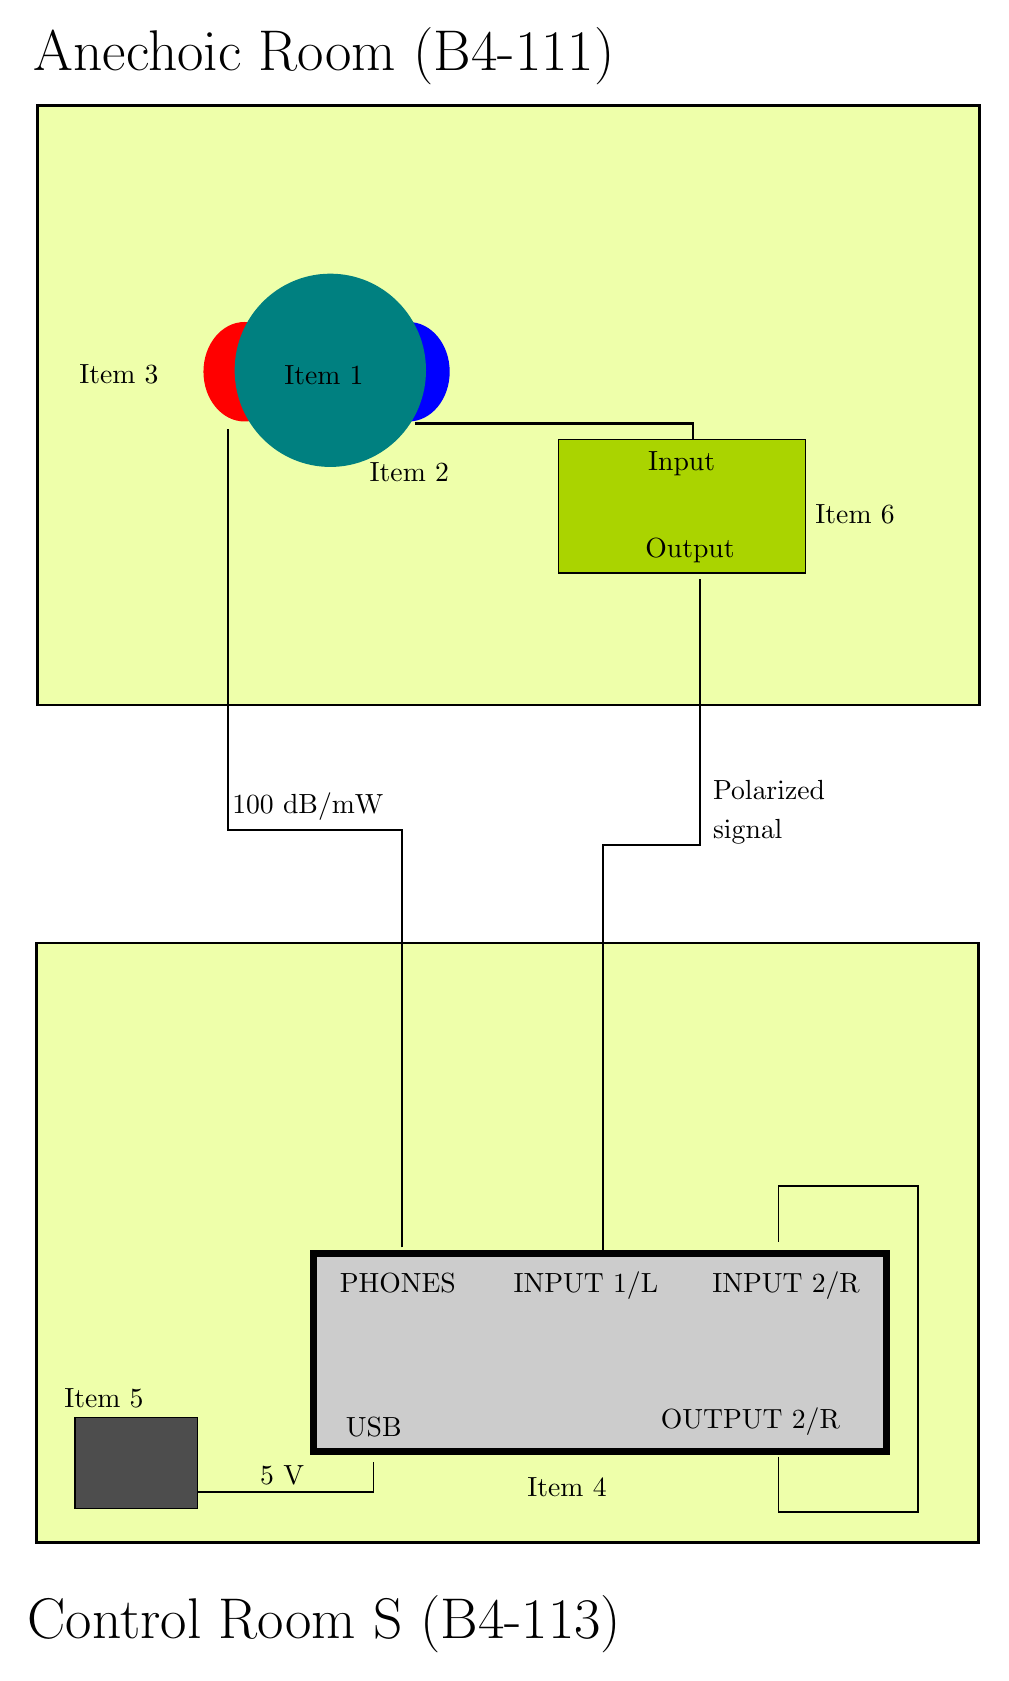
\begin{tikzpicture}[y=0.80pt, x=0.80pt, yscale=-1.000000, xscale=1.000000, inner sep=0pt, outer sep=0pt]
\begin{scope}% layer1
  \begin{scope}[shift={(-14.22335,105.14748)}]% layer1-7
    % rect3342
    \path[draw=black,fill=ceeffaa,line join=miter,line cap=butt,even odd rule,line
      width=0.968pt,rounded corners=0.0000cm] (160.5802,93.3428) rectangle
      (586.0658,364.2491);

    % path3348-0
    \path[fill=c0000ff] (328.0701,213.6738) ellipse (0.5225cm and 0.6318cm);

    % path3348-0-0
    \path[fill=cff0000] (254.0175,213.6738) ellipse (0.5225cm and 0.6318cm);

    % text3399
    \path[fill=black,line join=miter,line cap=butt,line width=0.800pt]
      (158.8386,84.1497) node[above right] (text3399) {\huge{Anechoic Room (B4-111)}};

    % path3350-7
    \path[fill=c008080] (292.7422,213.0265) ellipse (1.2151cm and 1.2272cm);

    % text3494
    \path[fill=black,line join=miter,line cap=butt,line width=0.800pt]
      (272.0000,219.3622) node[above right] (text3494) {Item 1};

    % text3520
    \path[fill=black,line join=miter,line cap=butt,line width=0.800pt]
      (179.3521,219.0369) node[above right] (text3520) {Item 3};

    % text3524
    \path[fill=black,line join=miter,line cap=butt,line width=0.800pt]
      (310.5353,263.3546) node[above right] (text3524) {Item 2};

    % text4346
    \path[fill=black,line join=miter,line cap=butt,line width=0.800pt]
      (515.8203,272.6747) node[above right] (text4346) {};

    % rect3342-0
    \path[draw=black,fill=ceeffaa,line join=miter,line cap=butt,even odd rule,line
      width=0.968pt,rounded corners=0.0000cm] (159.9447,471.6903) rectangle
      (585.4303,742.5966);

    % text3399-2
    \path[fill=black,line join=miter,line cap=butt,line width=0.800pt]
      (156.0388,792.2573) node[above right] (text3399-2) {\huge{Control Room S (B4-113)}};

    % text4387
    \path[fill=black,line join=miter,line cap=butt,line width=0.800pt]
      (285.9375,785.1747) node[above right] (text4387) {};

    % rect4395
    \path[draw=black,fill=ccccccc,line width=2.558pt,rounded corners=0.0000cm]
      (285.0705,611.9925) rectangle (543.8727,701.3781);

    % rect4397
    \path[draw=black,fill=c4d4d4d,line width=0.507pt,rounded corners=0.0000cm]
      (177.3497,685.9109) rectangle (232.6891,727.0794);

    % text4401
    \path[fill=black,line join=miter,line cap=butt,line width=0.800pt]
      (172.6317,681.3109) node[above right] (text4401) {Item 5};

    % text4405
    \path[fill=black,line join=miter,line cap=butt,line width=0.800pt]
      (381.7714,721.5567) node[above right] (text4405) {Item 4};

    % text4409
    \path[fill=black,line join=miter,line cap=butt,line width=0.800pt]
      (299.7695,694.7996) node[above right] (text4409) {USB};

    % path4417
    \path[draw=black,line join=miter,line cap=butt,even odd rule,line width=0.428pt]
      (232.8075,719.6862) -- (312.1120,719.6862) -- (312.1120,705.9801);

    % text5031
    \path[fill=black,line join=miter,line cap=butt,line width=0.800pt]
      (261.0862,716.0892) node[above right] (text5031) {5 V};

    % text5035
    \path[fill=black,line join=miter,line cap=butt,line width=0.800pt]
      (297.0000,629.3622) node[above right] (text5035) {PHONES};

    % path5039
    \path[draw=black,line join=miter,line cap=butt,even odd rule,line width=0.689pt]
      (324.9365,609.1651) -- (324.9365,420.7478) -- (246.6966,420.7478) --
      (246.6966,239.4242);

    % text5315
    \path[fill=black,line join=miter,line cap=butt,line width=0.800pt]
      (248.4749,416.5442) node[above right] (text5315) {100 dB/mW};

    % text5319
    \path[fill=black,line join=miter,line cap=butt,line width=0.800pt]
      (375.5305,632.6974) node[above right] (text5319) {INPUT 1/L};

    % text5319-3
    \path[fill=black,line join=miter,line cap=butt,line width=0.800pt]
      (465.2651,632.7798) node[above right] (text5319-3) {INPUT 2/R};

    % text7847
    \path[fill=black,line join=miter,line cap=butt,line width=0.800pt]
      (442.0128,693.9413) node[above right] (text7847) {OUTPUT 2/R};

    % path7851
    \path[draw=black,line join=miter,line cap=butt,even odd rule,line width=0.684pt]
      (495.1485,703.8376) -- (495.1485,728.7909) -- (558.3474,728.7909) --
      (558.3474,581.4711) -- (495.1485,581.4711) -- (495.1485,606.8978);

    % rect10551
    \path[draw=black,fill=caad400,rounded corners=0.0000cm] (395.6139,244.4652)
      rectangle (507.3367,304.5693);

    % text11321
    \path[fill=black,line join=miter,line cap=butt,line width=0.800pt]
      (511.8738,282.2976) node[above right] (text11321) {Item 6};

    % text11329
    \path[fill=black,line join=miter,line cap=butt,line width=0.800pt]
      (436.3157,260.5778) node[above right] (text11329) {Input};

    % text11333
    \path[fill=black,line join=miter,line cap=butt,line width=0.800pt]
      (435.0484,299.9692) node[above right] (text11333) {Output};

    % path3438
    \path[draw=black,line join=miter,line cap=butt,even odd rule,line width=0.640pt]
      (415.8100,610.3939) -- (415.8100,427.3141) -- (459.6653,427.3141) --
      (459.6653,307.0693);

    % text3440
    \path[fill=black,line join=miter,line cap=butt,line width=0.800pt]
      (465.6179,406.9453) node[above right] (text3440) {Polarized};
    % text3440

    \path[fill=black,line join=miter,line cap=butt,line width=0.800pt]
    (465.6179,426.9453) node[above right] (text3440) {signal};


    % path3446
    \path[draw=black,line join=miter,line cap=butt,even odd rule,line width=0.758pt]
      (330.9389,237.0558) -- (456.6796,237.0558) -- (456.6796,244.1533);

  \end{scope}
\end{scope}
\end{tikzpicture}
}